%!TEX root = curso_EDA_SLIDES.tex
%!TeX spellcheck = pt_BR
\section{Filas}

\begin{frame}

\begin{center}
{\Large Capítulo xxxxx -- Filas}
\end{center}

\begin{columns}
\begin{column}{.4\textwidth}
\centering
Pontos fundamentais a serem cobertos:
  \begin{enumerate}
  \item Contexto e motivação
  \item Definição
  \item Implementações
  \item Exercícios 
\end{enumerate}  

\end{column}
\begin{column}{.6\textwidth}
\centering
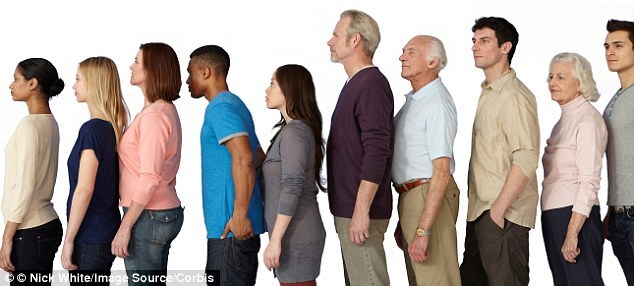
\includegraphics[height=4cm, width=7cm]{figs/fig_filas/fila_pessoas.jpeg}
%\hspace{+0.25cm}
%\scriptsize\textcolor{red}{[Tizio, Caio et al., Nature (2006)]}
\end{column}
\end{columns}


\end{frame}
%-----------------------------------------------------------------------


  \begin{frame}{Introdução}    

		\begin{itemize}
			\item Assim como a estrutura de dados Pilha, Fila é outra estrutura de dados bastante utilizada em computação.
			\item Um exemplo é a implementação de uma fila de impressão.
			\item Se uma impressora é compartilhada por várias máquinas, normalmente adota-se uma estratégia para determinar a ordem de impressão dos documentos.
			\item A maneira mais simples é tratar todas as requisições com a mesma prioridade e imprimir os documentos na ordem em que foram submetidos - o primeiro submetido é o primeiro a ser impresso.
		\end{itemize}
  \end{frame}

%-----------------------------------------------------------------------
  
\begin{frame}{Fila}
     \begin{block}{Definição}
       Um conjunto ordenado de itens a partir do qual podem-se eliminar itens numa extremidade (chamada de \alert{início} da fila) e no qual podem-se inserir itens na outra extremidade (chamada \alert{final} da fila).
     \end{block}          
\end{frame}

%-----------------------------------------------------------------------

\begin{frame}{Representação}
\begin{itemize}
	\item Os nós de uma fila são armazenados em endereços contínuos.	
	\item A Figura~\ref{fig:fila-representacao} ilustra uma fila com três elementos.
\end{itemize}
\begin{figure}[ht]
				\centering
				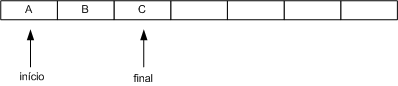
\includegraphics[width=.6\textwidth]{exemplo_fila_tres_elementos}
				\caption{Exemplo de representação de fila.}\label{fig:fila-representacao}
			\end{figure} 
\begin{itemize}
	\item Após a retirada de um elemento (\textit{primeiro}) temos:
	\begin{figure}[ht]
				\centering
				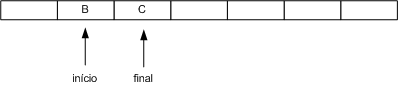
\includegraphics[width=.6\textwidth]{exemplo_fila_tres_retirada}
				\caption{Representação de uma fila após a remoção do elemento ``A''.}	
			\end{figure} 
\end{itemize}
\end{frame}
%-----------------------------------------------------------------------


\begin{frame}{Representação}
\begin{itemize}
	\item Após a inclusão de dois elementos temos:
	\begin{figure}[ht]
				\centering
				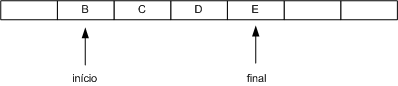
\includegraphics[width=.6\textwidth]{exemplo_fila_tres_inclusao}
				\caption{Representação de uma fila após a inclusão de dois elementos ``D'' e ``E''.}	
			\end{figure} 
\end{itemize}
\begin{itemize}
	\item Como podemos observar, a operação de inclusão e retirada de um item da fila incorre na mudança do endereço do ponteiro que informa onde é o início e o término da fila.
\end{itemize}
\end{frame}

\begin{frame}[fragile]{Representação}
\begin{itemize}
	\item Em uma fila, o \alert{primeiro} elemento inserido é o primeiro a ser removido.
	\item Por essa razão, uma fila é chamada \textbf{\alert{fifo(\textit{first-in first-out})}} -- primeiro que entra é o primeiro a sair -- ao contrário de uma pilha que é \alert{lifo} (\textit{last-in, first-out})
	\item Para exemplificar a implementação em C, vamos considerar que o conteúdo armazenado na fila é do tipo inteiro.
	\item A estrutura de fila possui a seguinte representação:	
\end{itemize}
\footnotesize
\begin{lstlisting}[language=C]
  struct fila{
    int elemento[N];
    int ini, n;
  }
  typedef struct fila Fila;
\end{lstlisting}

\begin{itemize}
	\item Trata-se de uma estrutura heterogênea constituída de membros distintos entre si. Os membros são as variáveis \alert{\textit{ini}} e \alert{\textit{fim}}, que serve para armazenar respectivamente, o início e o fim da fila e o vetor \alert{\textit{elemento}} de inteiros que armazena os itens da fila.
\end{itemize}
\end{frame}

\begin{frame}{Operações Primitivas}
  \begin{itemize}
	  \item As operações básicas que devem ser implementadas em uma estrutura do tipo Fila são:		
  \end{itemize}
  \begin{table}[ht]
			  \centering
						\begin{tabular}{l|l}
						    \hline \textbf{Operação} & \textbf{Descrição} \\
						    \hline criar() & aloca dinamicamente a estrutura da fila.\\
						    \hline insere(f,e) & adiciona um novo elemento \textit{(e)}, no final da fila \textit{f}.\\
						    \hline retira(f) & remove o elemento do início da fila \textit{f}.\\						   
						    %\hline pesquisar(f,e) & pesquisa o elemento \textit{e} na fila \textit{f}.\\
						    \hline 
						\end{tabular}
						\caption{Operações básicas da estrutura de dados fila.}
				\end{table}
\end{frame}
 
\begin{frame}{Operações auxiliares}   
			\begin{itemize}
				\item Além das operações básicas, temos as operações ``auxiliares''. São elas:
			\end{itemize}
			\begin{table}[ht]
			  \centering
						\begin{tabular}{l|l}
						    \hline \textbf{Operação} & \textbf{Descrição} \\						    
						    \hline vazia(f) & informa se a fila está ou não vazia.\\
						    \hline libera(f) & destrói a estrutura, e assim libera toda a memória alocada.\\
						    \hline 
						\end{tabular}
						\caption{Operações auxiliares da estrutura de dados fila.}
				\end{table}
  \end{frame}


\begin{frame}[fragile,plain]{Interface do Tipo Fila}
\footnotesize
\begin{lstlisting}[language=C]
typedef struct fila Fila;
/* Aloca dinamicamente a estrutura Fila, inicializando seus
 * campos e retorna seu ponteiro. A fila depois de criada
 * estarah vazia.*/
Fila* criar(void);

/* Insere o elemento e no final da fila f, desde que,
 * a fila nao esteja cheia.*/
void insere(Fila* f, int e);

/* Retira o elemento do inicio da fila, e fornece o 
 * valor do elemento retirado como retorno, desde que a fila
 * nao esteja vazia*/
int retira(Fila* f);

/*Verifica se a fila f estah vazia*/
int vazia(Fila* f);

/*Libera a memoria alocada pela fila f*/
void libera(Fila* f);
\end{lstlisting}
\end{frame}

\begin{frame}{Implementação de Fila com Vetor}
	\begin{itemize}
		\item Assim como nos casos da pilha e lista, a implementação de fila será feita usando um vetor para armazenar os elementos.
		\item Isso implica, que devemos fixar o número máximo de elementos na fila.
		\item O processo de inserção e remoção em extremidades opostas fará a fila ``andar'' no vetor.
		\item Por exemplo, se inserirmos os elementos 8, 7, 4, 3 e depois retiramos dois elementos, a fila não estará mais nas posições iniciais do vetor.
	\end{itemize}
	\begin{figure}[ht]
				\centering
				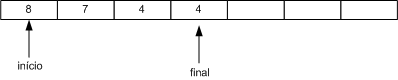
\includegraphics[width=.6\textwidth]{fila_insercao_quatro_elementos}
				\caption{Fila após inserção de quatro elementos.}	
	\end{figure} 	
\end{frame}

\begin{frame}{Implementação de Fila com Vetor}	
	\begin{figure}[ht]
				\centering
				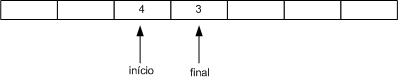
\includegraphics[width=.6\textwidth]{exemplo_fila_remove_dois_elementos}
				\caption{Fila após retirar dois elementos.}	
	\end{figure} 	
	\begin{itemize}
		\item Com essa estratégia, é fácil observar que, em um dado instante, a parte ocupada pelo vetor pode chegar a última posição.
		\item Uma solução seria ao remover um elemento da fila, deslocar a fila inteira no sentido do início do vetor.
		\item Entretanto, essa método é bastante ineficiente, pois cada retirada implica em deslocar cada elemento restante da fila. Se uma fila tiver 500 ou 1000 elementos, evidentemente esse seria um preço muito alto a pagar.		
	\end{itemize}
\end{frame}

\begin{frame}{Implementação de Fila com Vetor}		
	\begin{itemize}		
		\item Para reaproveitar as primeira posições do vetor sem implementar uma ``re-arrumação'' dos elementos, podemos incrementar as posições do vetor de forma ``circular''.
		\item Para essa implementação, os índices do vetor são incrementados de maneira que seus valores progridam ``circularmente''. 
		\item Dessa forma, se temos 100 posições no vetor, os índices assumem os seguintes valores:
		$$0, 1, 2, 3, \cdots, 98, 99, 0, 1, 2, 3, \cdots, 98, 99, \cdots$$
	\end{itemize}
\end{frame}

\begin{frame}[fragile]{Função de Criação}
	\begin{itemize}
		\item A função que cria uma fila, deve criar e retornar o ponteiro de uma fila vazia;
		\item A função deve informar onde é o início da fila, ou seja, fazer $f->ini = 0$, como podemos ver no código abaixo.
		\item A complexidade de tempo para criar a fila é constante, ou seja, $O(1)$.
	\end{itemize}
\small	
\begin{lstlisting}[language=C]
/* Aloca dinamicamente a estrutura Fila, inicializando seus
 * campos e retorna seu ponteiro. A fila depois de criada
 * estarah vazia.
 */
Fila* criar(void)
{
   Fila* f = malloc(sizeof(Fila));
   f->n = 0;
   f->ini = 0;
   return f;
}
\end{lstlisting}
\end{frame}

\begin{frame}[fragile]{Função de Inserção}  
	\begin{itemize}
		\item Para inserir um elemento na fila, usamos a próxima posição livre do vetor, indicada por \alert{n}.
		\item Devemos assegurar que há espaço para inserção do novo elemento no vetor, haja vista se tratar de um vetor com capacidade limitada. 
		\item A complexidade de tempo para inserir um elemento na fila é constante, ou seja, $O(1)$.
	\end{itemize}
\footnotesize
\begin{lstlisting}[language=C]
/* Insere o elemento e no final da fila f.*/
void insere(Fila* f, int e)
{
  int fim;
  if (f->n == N){
     printf("Fila cheia!\n");
  }else{
     fim = (f->ini + f->n) % N;
     f->elementos[fim] = e;  
     f->n++;
  }
}
\end{lstlisting}	
\end{frame}

\begin{frame}[fragile]{Função de Remoção} 
	\begin{itemize}
		\item A função para retirar o elemento do início da fila fornece o valor do elemento retirado como retorno.
		\item Para remover um elemento, devemos verificar se a fila está ou não vazia.
		\item A complexidade de tempo para remover um elemento da fila é constante, ou seja, $O(1)$.
	\end{itemize}
	
\footnotesize
\begin{lstlisting}[language=C]
int retira(Fila* f)
{
  int e;
  if (vazia(f))
    printf("Fila vazia!\n");
  else{
    e = f->elementos[f->ini];
    f->ini = (f->ini + 1) % N;
    f->n--;
  }
  return e;
}
\end{lstlisting}	
\end{frame} 

%\begin{frame}[fragile]{Função de Pesquisa} 
%	\begin{itemize}
%		\item Para pesquisar um elemento qualquer na lista é necessário compará-lo com os elementos existentes, utilizando alguns dos algoritmos de busca conhecidos;
%		\item A complexidade de tempo dessa função depende do algoritmo de busca implementado. Se utilizarmos a busca seqüencial, a complexidade da função será $O(n)$. No entanto, é possível baixá-lo para $O(n\log n)$, utilizando alguns dos algoritmos mais refinados.
%\end{itemize}
%
%\footnotesize
%\begin{verbatim}
%}\end{verbatim}
%\end{frame}

\begin{frame}[fragile]{Exemplo de Uso da Fila}

\begin{footnotesize}

\begin{lstlisting}[language=C]
#define N 10
#include <stdio.h>
#include "fila.h"

int main(void)
{
    Fila* f = criar();
    
    int i;
    for (i = 0; i < N; i++)
      insere(f,i * 2);
      
    printf("\nElementos removidos: ");
      
    for (i = 0; i < N/2; i++)
     printf("%d ", retira(f)); 
               
    system("pause");    
}
\end{lstlisting}
\end{footnotesize}
\end{frame} 


\begin{frame}{Referências}
	
	\begin{enumerate}
		\item Tenenbaum, A. M., Langsam, Y., and Augestein, M. J. (1995). Estruturas de Dados Usando C. MAKRON Books, pp. 207-250.
		\item Wirth, N. (1989). Algoritmos e Estrutura de dados. LTC, pp. 151-165.
	
	\end{enumerate}
	
\end{frame}
